%%% DOCUMENT SETUP %%%
\documentclass[11pt,a4paper,onecolumn]{article}
\usepackage[english]{babel}

%%% LAYOUT %%%
\usepackage{fullpage}
\usepackage[a4paper]{geometry}
\usepackage[parfill]{parskip}
\usepackage{multicol}
\usepackage{footnote}

%%% GRAPHICS %%%
\usepackage{graphicx}
\usepackage{color}
\usepackage{graphics}
\usepackage{rotating}
\usepackage{subfig}
\usepackage{amsmath}
\usepackage{amssymb}
\usepackage{amscd}
\usepackage{xfrac}
\usepackage{float}
\usepackage{dsfont}

%%% FONT %%%
\usepackage{ifxetex}
\ifxetex
  \usepackage{fontspec}
    \setmainfont{Linux Libertine O}
  \usepackage{xunicode}
  \usepackage{microtype}
\else
  \usepackage[T1]{fontenc}
  \usepackage[latin1]{inputenc}
  \usepackage{times}
  \usepackage{microtype}
\fi

%%% Coding %%%
\usepackage{listings}
\usepackage{pseudocode}

%%% TITLE PAGE %%%
\author{Jeroen Hofman (10194754) \\
[15pt] University of Amsterdam (\textsc{UvA})}

\title{Concurrent Programming week 4:\\
  MPI
		}

\begin{document}
\maketitle
\captionsetup{width=0.8\textwidth}
\lstset{language=C,breaklines=true,backgroundcolor=\color{white},frame=none,basicstyle=\footnotesize}
\thispagestyle{empty}

%%% ABSTRACT %%%
\begin{center}
\begin{abstract}
\small{We implemented the heat diffusion problem with MPI and found significant speedups up to a factor of 22 for 4 nodes (32 cores) on LISA. We found linear scaling for big matrix sizes and decreasing performance for small matrix sizes when using multiple nodes. We also bench-marked the system on LISA using MPI and we found values for the bandwidth and latency in the expected range. Next we implemented three different versions of broadcasting a message in MPI, where a version using a cascade of messages was found to achieve good performance relative to the original implementation of \texttt{MPI\_Bcast}.}
\end{abstract}
\end{center}

%%% TABLE OF CONTENTS %%%
\newpage
\tableofcontents
\newpage

\section{Heat diffusion with MPI}
\subsection{Algorithm}
In this report we implement the heat diffusion problem with MPI. The code is available in /mpi/compute.c. The setup is slightly different compared to the previous weeks. At the beginning of the program we initialize the processes, and give the processes an id. Every process is given a part of the temperature matrix to compute, divided in the row direction, like the previous two weeks. Every process gets a number of rows which is roughly equal to the number of rows in the temperature matrix divided by the number of threads, where the maximum difference from the actual assigned number of rows and this calculation is 1, so the workload is equally balanced. After the workload is divided every process gets its own two temperature arrays and its own conductivity array which has the same size as the chunk the process has obtained in the scheduling. This is different from previous week since we have no shared memory here. The temperature arrays and the conductivity arrays are then initialized to the correct values, where every process has to do the initialization separately. Every process obtains a halo row both at the bottom and the top of its matrix, containing the same values as the top and bottom row of its neighboring processes, because we need the top and bottom neighbor for the computation of the new temperature values.

After initialization the master process (in this case always the process with id 0) will start a timer after all processes have hit a barrier, this is to ensure all processes are done with initialization. Every process then enters the main loop and first enters the loop for the main computation, i.e. the filling of the new temperature matrix and the calculation of the local temperature difference.
 
This part is different from previous weeks, since we first compute the first and last row of every chunk (not the halo rows), before computing the rest of the matrix. After having computed the first and last row and having copied the values to the halo elements in the first and last column corresponding to these rows to implement the continuous boundary condition we initialize sending the top and bottom row to the neighbor processes by calling the non-blocking \texttt{MPI\_Isend}. We also initiate receiving the last row from the previous process and the first row from the next process to copy them in the halo rows with the non-blocking  \texttt{MPI\_Irecv}. We can do this since all necessary data has already been computed. It is important that processes can both read and write at the same time, because of limited buffer sizes, i.e. for large matrices one row does not fit entirely in the buffer and so if all processes start sending first with a blocking function call they will deadlock, because they cannot finish and will all wait for the receiving process to take data out of the buffer, which it cannot, since it is in a blocking sending function call itself. After the message sending has been initiated the processes continue with calculating the rest of the new matrix and the local temperature difference and when this is completed the copying of the columns to the halo columns takes place. 

After completing the copying the processes call \texttt{MPI\_Allreduce} to calculate a global maximum temperature difference. The processes need the global maximum temperature difference to check whether or not the threshold is reached, which is done in the beginning of the loop. 

The function calls \texttt{MPI\_Isend} and \texttt{MPI\_Irecv} called before are non-blocking, so the processes do not suspend in the functions while waiting for completion, but execute both functions and then suspend in a \texttt{MPI\_Wait} where they return from when the sending and receiving has been completed. This \texttt{MPI\_Wait} functions are called in this point of the computation, where this part also acts like an implicit barrier, since all threads should have finished sending and receiving messages before they continue.

Next if the current iteration is a multiple of the reporting frequency, the local maximum, minimum and average are obtained as well. The local maximum, minimum and average temperature are sent to the master thread and compared to compute the global variable via a \texttt{MPI\_Reduce} clause, where they are directly written to the report struct of the master thread. The local temperature difference is written to all threads via \texttt{MPI\_Allreduce}, however this is not strictly needed for reporting purposes. The \texttt{MPI\_Reduce} and \texttt{MPI\_Allreduce} act as a barrier and after all processes have written their values, the master thread reports them.

Since the processes can only continue when they are finished receiving and sending the data they can safely swap the pointers of the temperature matrices after wards (or after the reporting) and continue entering the next iteration, if the maximum number of iterations is not reached or the global maximum difference is above the threshold.

Another way to implement the sending and receiving of the data would be to initialize the send and receive procedures before entering the loop with \texttt{MPI\_Send\_init} and \texttt{MPI\_Recv\_init} and then start these function calls with \texttt{MPI\_Start} or \texttt{MPI\_Startall} for all four (or two) of the required function calls. The \texttt{MPI\_Start} routine is essentially equal to \texttt{MPI\_Isend} (so non-blocking) and after wards the processes will call \texttt{MPI\_Wait} just as above. This method has the advantage that the initialization of the message sending and receiving only has to be done once. However, this method does not work since the buffer which is given as argument in \texttt{MPI\_Send\_init} and \texttt{MPI\_Recv\_init} is assumed to be static in terms of its memory address, while in our case the pointers of these matrices are swapped every iteration and hence the buffer address is not constant.

The amount of barriers in this implementation is effectively only one, namely at the \texttt{MPI\_Allreduce} before the sending and receiving of messages starts. This is an advantage of non-shared memory models, since in the case of PThreads we needed two barriers and in the case of OpenMP we needed three barriers. Note however there is some kind of semi-barrier invoked by the \texttt{MPI\_wait} function calls, since the process cannot advance further in the code from this point until its two 'neighboring' processes are at least also at this point. This is not a complete synchronization but it does make sure the processes have to be in the same section of code.

\subsection{Results}
We measured the total execution time and the FLOP/s for different number of processes. On one node (with 8 cores) we measured the performance from 1 to 8 processes, on 2 nodes we measured the performance for 12 and 16 processes, on 3 nodes for 24 processes and on 4 nodes for 32 processes. The measurements are hence a little different from previous weeks. All measurements were repeated 3 times and the minimum execution time or maximum FLOP/s is reported here. The FLOP/s are calculated from the standard macro provided in the skeleton. The numerical results are given in Table \ref{tab:heat} and the relative speedups are given in Figure \ref{fig:heat}.
 
\begin{figure}[H]
 \centering
  \subfloat{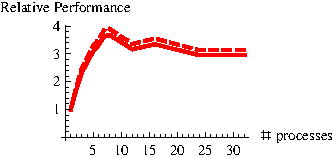
\includegraphics[width=0.33\textwidth]{100.pdf}}
  \subfloat{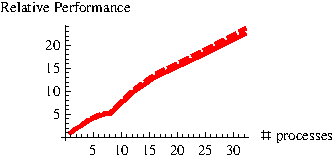
\includegraphics[width=0.33\textwidth]{1000.pdf}}
  \subfloat{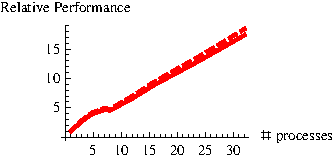
\includegraphics[width=0.33\textwidth]{5000.pdf}}
  \caption{Relative performance results for matrix sizes 100x100 (left), 1000x1000 (middle) and 5000x5000 (right). The solid line has the sequential code as baseline, the dashed line has the MPI code with 1 process as baseline.}
  \label{fig:heat}
\end{figure}

\begin{table}[H]
  \centering
  \begin{tabular}{l | c | l | c | l }
    \# threads & Execution time & FLOP/s & Execution time & FLOP/s \\
    \hline
    \multicolumn{1}{c}{} & \multicolumn{2}{| c |}{Size 100x100 ($10^6$ iterations)} & \multicolumn{2}{c}{Size 1000x1000}\\
    \hline
    seq. code & 5.3130341 & 2.258596 $10^9$ & 6.353987 & 1.888578 $10^9$ \\
    1 & 4.679846 & 2.127173 $10^9$ & 6.687384 & 1.794424 $10^9$ \\
    2 & 2.549025 & 3.905352 $10^9$ & 3.360593 & 3.570798 $10^9$ \\
    3 & 1.881140 & 5.302972 $10^9$ & 2.478653 & 4.841339 $10^9$ \\    
    4 & 1.600307 & 6.170246 $10^9$ & 1.836402 & 6.534517 $10^9$ \\
    5 & 1.423424 & 6.993587 $10^9$ & 1.564210 & 7.671604 $10^9$ \\
    6 & 1.321645 & 7.532159 $10^9$ & 1.384143 & 8.669625 $10^9$ \\
    7 & 1.206728 & 8.249448 $10^9$ & 1.273523 & 9.422680 $10^9$ \\
    8 & 1.199771 & 8.297283 $10^9$ & 1.254324 & 9.566906 $10^9$ \\
    12 & 1.390424 & 7.159572 $10^9$ & 0.659500 & 18.19560 $10^9$ \\
    16 & 1.315322 & 7.568367 $10^9$ & 0.489642 & 24.50770 $10^9$ \\
    24 & 1.490888 & 6.677121 $10^9$ & 0.362961 & 33.06140 $10^9$ \\
    32 & 1.442690 & 6.6900193 $10^9$ & 0.284789 & 42.13646 $10^9$ \\
    \hline
    \multicolumn{1}{c}{} & \multicolumn{2}{| c |}{Size 20000x500} & \multicolumn{2}{c}{Size 500x20000}\\
    \hline
    seq. code & 63.647849 & 1.885374 $10^9$ & 65.108231 & 1.843085 $10^9$ \\
    1 & 66.666906 & 1.799935 $10^9$ & 67.81081 & 1.769629 $10^9$ \\
    2 & 34.50418 & 3.477839 $10^9$ & 35.23763 & 3.405451 $10^9$ \\
    3 & 23.99135 & 5.001804 $10^9$ & 25.01105 & 4.797880 $10^9$ \\
    4 & 19.19551 & 6.251463 $10^9$ & 20.09395 & 5.971948 $10^9$ \\
    5 & 16.08525 & 7.460250 $10^9$ & 16.95278 & 7.074840 $10^9$ \\
    6 & 14.93507 & 8.034778 $10^9$ & 15.68000 & 7.653060 $10^9$ \\
    7 & 15.02547 & 7.986437 $10^9$ & 14.33389 & 8.368814 $10^9$ \\
    8 & 14.39780 & 8.334604 $10^9$ & 14.76351 & 8.128150 $10^9$ \\
    12 & 9.417766 & 12.74188 $10^9$ & 9.957370 & 12.05138 $10^9$ \\
    16 & 7.240649 & 16.57310 $10^9$ & 7.716900 & 15.55029 $10^9$ \\
    24 & 4.806864 & 24.96430 $10^9$ & 5.385971 & 22.28011 $10^9$ \\
    32 & 3.654067  & 32.84012 $10^9$ & 4.310615 & 27.83826 $10^9$ \\
    \hline
    \multicolumn{1}{c}{} & \multicolumn{2}{| c |}{Size 5000x5000} & \multicolumn{2}{c}{}\\
    \hline
    seq. code & 155.836412 & 1.925096 $10^9$ & & \\
    1 & 165.2869 & 1.815026 $10^9$ & & \\
    2 & 83.4971 & 3.607950 $10^9$ & & \\
    3 & 57.03851 & 5.259604 $10^9$ & & \\
    4 & 45.19727 & 6.637467 $10^9$ & & \\
    5 & 38.60983 & 7.770133 $10^9$ & & \\
    6 & 36.07402 & 8.316234 $10^9$ & & \\
    7 & 34.49512 & 8.968567 $10^9$ & & \\
    8 & 34.30923 & 8.744002 $10^9$ & & \\
    12 & 23.610953 & 12.70597 $10^9$ & & \\
    16 & 17.423131 & 17.21849 $10^9$ & & \\
    24 & 11.960893 & 25.08147 $10^9$ & & \\
    32 & 8.977228 & 33.41789 $10^9$ & & \\
  \end{tabular}
  \caption{Results for the MPI code for heat diffusion for different matrix sizes and number of processes.}
  \label{tab:heat}
\end{table}

Starting with the smallest matrix performance increases linearly up to 7 processes on 1 node. Using multiple processes has no effect on performance, this is caused by the increased overhead of communication between nodes and the relatively small matrix size. If we use the matrix of 1000x1000 however we see a significant increase in performance up to 32 cores, the only measurement where performance does not increase is between 7 and 8 cores per node. However, the LISA manual also suggests that running one process less per node can be advantageous because one core can be used for scheduling and other OS tasks at that point. However, this effect only occurs with one node, for multiple nodes setting the number of processes to 14 or 15 gives worse performance than 16 processes, and the same holds for 24 and 32 processes, when decreasing this numbers by 1 or the number of active nodes. For a matrix size of 1000x1000 we find a maximum speedup of a factor 22 with the sequential code as baseline with 32 processes (23 with the MPI code with 1 process as baseline), so there is a substantial amount of overhead present in this case, since we have around 70\% efficiency. This overhead increases with the number of nodes that is involved, since for 16 processes (2 nodes) we find a speedup of roughly a factor 14 (87.5\% efficiency) and for 24 processes we find a speedup of a factor 18.5 (77\% efficiency)

If we look at the matrices of sizes 500x20000 and 20000x500 we see a similar speedup, though less than for the 1000x1000 matrix. If we use a matrix of 20000x500 we have a somewhat better performance compared to 500x20000, this is because of the smaller rows and hence the reduction in message sizes between processes. This difference however only occurs with more than one node (more than 8 processes), indicating that maybe if the processes are on one node they do not exchange the full message, but rather just the pointers, since they have access to the same shared memory. This will be further discussed in the next section. The reason that the speedup for both 20000x500 and 500x20000 is less pronounced than for 1000x1000 will be discussed in the next paragraph.

If we look at the last matrix size, 5000x5000, we see a more or less similar performance. A linear speedup, with a small constant zone around 7 and 8 processes. As in the case of 500x20000 and 20000x500 we do not reach the same speedups and performance as in the case of 1000x1000. A possible reason is that for 5000x5000 and 500x20000 the communication overhead is much larger since the rows are very long, however this does not explain the worse performance for the 20000x500 matrix compared to 1000x1000 since the message exchanging in that case is actually smaller. However, in this case cache locality might play a role, since first calculating the first and last row of a chunk of 20000 rows is very expensive and leads to poor performance in the cache. This effect is less pronounced in the case of 1000x1000 matrix for instance. This might explain the poor performance of the 20000x500 matrix compared to the 1000x1000 matrix. It is important to note that these differences in large matrices are much bigger when multiple nodes are involved, this probably has to do with the pointer exchange if the processes are on the same node, as mentioned above.

The maximum speed we achieve is 42.14 $10^9$ FLOP/s which is understandably much higher than in the case of PThreading (7.22 $10^9$) or OpenMP (7.08 $10^9$), since we cannot use multiple nodes in those cases. However it would be more fair to compare the maximum speed that is achieved for 8 processes on 1 node with the best performance of PThreading and OpenMP. We then find a value of 9.57 $10^9$ FLOP/s, which is much higher than the maximum speedups achieved for PThreading and OpenMP for 8 threads. A reason might be the decreased number of barriers for MPI, since we do not use shared memory. Next to this there is also no need for global variables like in the case of OpenMP which gave a significant performance decrease. The \texttt{MPI\_Reduceall} that replaces this task of writing to the global variable is much more efficient and does not use global variables internally probably. The messaging apparently also is very efficient, as this might give a possible decrease in performance compared to PThreads and OpenMP, but this does not happen (MPI is performing better along all matrix sizes and process numbers).

Next to this there is of course the advantage of using multiple nodes, which can further increase performance, though the overhead increases significantly.  

\section{Basic point to point communication}
As described in the assignment, we create a simple system where messages of arbitrary size are passed from one process to another. By passing very small messages we are able to give an approximation of the latency, if we assume the sending itself is nearly instant. By passing very big messages we can measure the bandwidth of a system. The passing of messages is done in a ring system where every process sends a message to the next, and the last process sends a message to a process with id 0. We tested the bandwidth and the latency with two different structures: one LISA node where the processes are all on the same node (inter-core communication) and two LISA nodes where the processes are on a different node (inter-node communication). In both cases we only use 2 processes.

The algorithm for this problem is very simple (the code is given in mpi/benchmark.c), process 0 starts sending a message initialized with \texttt{MPI\_Send\_init} with \texttt{MPI\_Start} and suspends in a \texttt{MPI\_Wait}. After it has returned from the \texttt{MPI\_Wait} it will initiate a \texttt{MPI\_Start} for the \texttt{MPI\_Recv\_Init} and suspend in a \texttt{MPI\_Wait}. The other processes will do the same but start with a \texttt{MPI\_Start} for the \texttt{MPI\_Recv\_Init} first and will then start with an \texttt{MPI\_Start} for the \texttt{MPI\_Send\_init} since otherwise the system will reach a deadlock and we want to achieve circular message passing.  

For the latency we used $10^6$ iterations and a message size equal to the size of a \texttt{char}, on most systems this is 1 byte. Calling the program is done by \texttt{mpiexec -n <number of processes> benchmark <number of iterations> <message size in bytes>}. For the bandwidth measurement we used 100 iterations and a message size of 100 MB (message sizes larger than this value do not change the result). The results are the minimum latency and maximum bandwidth for a total of 3 runs, the results are given in the Table \ref{tab:point} below.

\begin{table}[H]
  \centering
  \begin{tabular}{l | l | l }
    & Inter-node & Inter-core \\
    \hline
    Latency (s) & 1.93 $10^{-6}$ & 7.04 $10^{-7}$\\
    Bandwidth (MB/s) & 1.43 $10^3$ & 1.46 $10^3$\\
  \end{tabular}
  \caption{Latency and bandwidth measurements on LISA, both for inter-node (left) and inter-core (right).}
  \label{tab:point}
\end{table}

The results shown above are in line with system specifications provided by \cite{LISA}. When communication is performed between nodes the system that is used is Infiniband, which has a bandwidth of 1.6 GB/s and a latency smaller then 6 $10^{-6}$ s. We see indeed from our measurements that this is the case. We measure only 90\% of the bandwidth which is given in the documentation, this is probably because of overhead by the invoking of some protocols for data sending and some system specific settings which we cannot, or do not have time to, adjust. Also the code itself provides overhead by calling MPI functions repeatedly, though this has been minimized by using \texttt{MPI\_Recv\_init} and \texttt{MPI\_Send\_init}.

The measurements for inter-core are disputable, since MPI might be smart enough to simply pass a pointer, since it detects that the messages that are to be sent are on the same node and hence are in the same shared memory. However, for the latency this should not make much difference since we measure that by sending 1 byte anyway, and sending a pointer will be of the same order of magnitude in size. Hence our measurement of 704 nanoseconds might give a good indication of the latency between cores, although since this is very low, the overhead in the code might become significant and the actual speed of passing a pointer (or sending a message of 1 byte) might actually be much larger. Indeed, some sources like \cite{latency} report inter-core latencies of under 100 nanoseconds. The bandwidth in this case is completely unreliable since in the case of pointer passing we are not actually passing the message but just a pointer and hence the presumed message size of 100MB is false.

\section{OpenMP Features}
In this last section of the report we implement our own version of the \texttt{MPI\_Bcast} function, where one node broadcasts a message to all other nodes. For simplicity we assume this node to be always the node with id 0. We compare three versions all available in /mpi/broadcast\_test.c. The program can be called by \texttt{mpiexec -n <number of processes> broadcast\_test <number of iterations> <data size in bytes>} where \texttt{<number of iterations>} gives the number of times a broadcast should be performed.

\begin{itemize}
\item 
  Original version: We call \texttt{MPI\_Bcast} for the number of iterations provided above and measure the time it takes for a single broadcast to complete.
\item
  Simple version: The process with id 0 sends a message to all other nodes with \texttt{MPI\_Isend} and then calls a \texttt{MPI\_Waitall} after wards. All the other processes call a \texttt{MPI\_Recv}. After every iteration a \texttt{MPI\_Barrier} is called to make sure all processes are synchronized because the documentation on the handling of the above functions is a bit vague, and we want to make sure that every process is at the same iteration. This algorithm is repeated for the number of iterations provided above.
\item
  Cascade version: The broadcasting is divided into rounds, starting with round 0, where every round $2^{\text{round}}$ processes are sending a message to a process which did not receive a message yet. The message sending has a tree structure, an example with 4 processes:\\
  Round 0:\\
  - $0 \rightarrow 1$ (id 0 sends to id 1)\\
  - $1 \leftarrow 0$ (id 1 receives from id 0)\\
  Round 1:\\
  - $0 \rightarrow 2$\\
  - $1 \rightarrow 3$\\
  - $2 \leftarrow 0$\\
  - $3 \leftarrow 1$\\
To speed up the computation every round the processes that should send a message with \texttt{MPI\_Send} and the processes that should receive a message with \texttt{MPI\_Recv} are calculated with bit shifts, since we have arithmetic in a power of 2. We do not use \texttt{MPI\_Isend} since this requires implementing a \texttt{MPI\_Waitall} with parameters which have a dynamic size, and are not even constant per round, since the number of processes is not necessarily a power of two and so in the last round the workload might not be equally distributed. This also creates more overhead, while this implementation already has significant overhead due to branching. We repeat this again a number of iterations and we put a \texttt{MPI\_Barrier} at the end of every iteration to make sure all processes are synchronized. 
\end{itemize}

We tested these three methods on 8 nodes on LISA, with 1 process per node. We tested for different message sizes, ranging from 1 byte to approximately 100MB. The average execution time was measured over 1000 iterations, where the experiment was repeated three times. The results are given in Figure \ref{fig:broadcast}.

\begin{figure}[H]
  \centering
  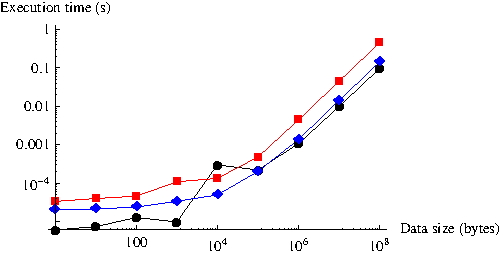
\includegraphics[width=0.7\textwidth]{broadcast.pdf}
  \caption{Execution time per broadcast as a function of message size. The black line is the original implementation, the red line is the simple version and the blue line is the cascade version.}
  \label{fig:broadcast}
\end{figure}

The figure shows that the original implementation gives the best performance. The cascade version performs better than the simple version and approaches the original implementation for large data sizes, indicating that probably the original implementation uses a similar cascade version and maybe switches to another approach for small data sizes, as the overhead produced by the cascade version is larger and hence becomes significant for small data sizes. The original implementation makes a strange jump from $10^3$ to $10^4$ bytes. This was the case in multiple experiments, it might be that this is the point where the routine switches between or uses a mix of algorithms which decreases performance in this area. It might also be the point at which the message is larger than the buffer size and so a significant jump in execution time occurs. Still it is strange that only at this particular size the original implementation performs worse at this point than the other versions.

\section{Conclusions}
We implemented a MPI version of the problem of heat diffusion and we found a significant speedup up to a factor of 22 when using 32 processes on 4 cores. The overhead produced by the message passing increases with the number of nodes. By using MPI we outperformed OpenMP and PThreads by almost 35\%, even when not taking into account the possibility of using multiple nodes. We also investigated the bandwidth and latency between LISA nodes and found values consistent of those provided by the LISA documentation. We also investigated the possibility that for inter-core message passing on the same node MPI might just pass pointers since both cores have access to the same shared memory. Lastly we looked at different implementations of a broadcast function, using the original implementation provided by MPI and using two other approaches only using primitives. It turned out that for large data sizes an approach which using a cascade of messages performed almost as well as the original implementation by MPI.

%%% BIBLIOGRAPHY %%%
\begin{thebibliography}{7}
\bibitem{LISA}
  http://sara.nl/systems/lisa/description
\bibitem{latency}
  http://mechanical-sympathy.blogspot.com/2011/08/inter-thread-latency.html
\end{thebibliography}

\end{document}
